\section{Theoretical Basics}
\label{sec:theoretical_basics}
\subsection{Basics of Tumor Biology}
\begin{figure}[h]
    \centering
    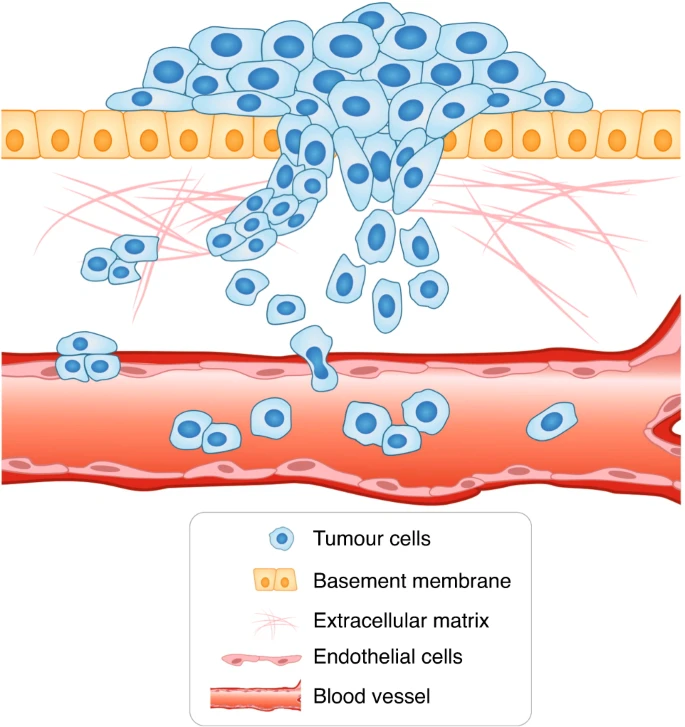
\includegraphics[width=0.85\textwidth]{resources/images/tumour_invasion_stage.png}
    \caption{Tumor Invasion Stage}
    \label{fig:tumor_invasion_stage}
\end{figure}

The body of a living creature is made up of more than 200 different types of cells; the coordination between the cells and their surroundings keeps the body running. Each of these cells is built from the genetic information encoded in the DNA in the cells' nuclei. Though the nucleotide sequence of DNA is well-checked and maintained throughout the cell's life, mutations still occur that cause changes in a cell's DNA. These mutations may be of a positive, negative, or neutral nature. In the case of a harmful mutation, this alternation of the DNA may cause diseases, with cancer being one of them. The failure of the complex system managing cell birth, proliferation, and cell death (apoptosis) causes cancer, resulting in uncontrolled cell proliferation in a local area. A conglomeration of cancer cells is called a tumor. 

Cancer diseases can be categorized medically into five stages. First is the tumor initiation phase, where it comes to the above explained genetic mutations of normal cells. The next stage is the tumor promotion stage, in which the mutated cells of phase one may experience further genetic alterations resulting from uncontrolled growth and proliferation of the cancerous cells. The third stage is the tumor progression stage, where the cancerous cells progress in growing and proliferating, reaching a critical mass, and forming a tumor at a local site of the body. Fourth comes the invasion stage, shown in figure~\ref{fig:tumor_invasion_stage}. Here, the tumor can invade surrounding tissue by breaking through the cellular membrane, invading the extracellular matrix inside, and entering the blood circulation or lymphatic systems. Next, the tumor cells that have invaded the blood circulation of the lymphatic system spread throughout the body and form new tumors. This stage is called Metastization. To grow tumors further, they need access to nutrients and oxygen. During angiogenesis, a tumor develops its own blood vessels, securing its nutritional provision. At this stage, the first symptoms of the host may appear, enabling medical treatment.

In our model, the focus lies on the first two stages: tumor invasion and tumor progression. The tumor invasion stage is characterized by the malignant cells gaining the ability to penetrate and invade the surrounding tissue. The tumor cells break through the normal tissue barrier and infiltrate neighboring structures. In order to do so, the cancer cells produce so-called matrix-degrading enzymes which break down the extracellular matrix. The degradation of the extracellular matrix helps local spreading and destroys otherwise healthy tissue and cells in the affected area. In the next phase, the tumor progression stage, the tumor has grown more extensive, and the cancerous cells take on more aggressive behavior by invading the surrounding area further. While they keep growing uncontrolled, they are also affected by further genetic instabilities, which lead to more mutations, possibly developing resistance mechanisms against, for example, degrading factors. Already in this stage, the affected area is exposed to heavy tissue damage and functional disabilities.

The most important factors influencing those two phases are the genetic dispositions of the tumor cells towards proliferation and the evasion of apoptosis, programmed cell death, which increase the invasive potential. Another critical factor is the geometry of the extracellular matrix, as well as the exact macromolecules that make it up. A solid immune biological defense reaction also helps the body defend against spreading cancer cells. Hence, evasion of detection and destruction of the tumor cells plays a vital role in the first stages. To invade the affected area, the malignant cells need to be able to move freely and quickly. In order to do so, cancer cells can gain the ability to lose adhesion properties, which healthy cells usually have, to allow migrating into the surrounding tissue.
\begin{figure}[h]
    \centering
    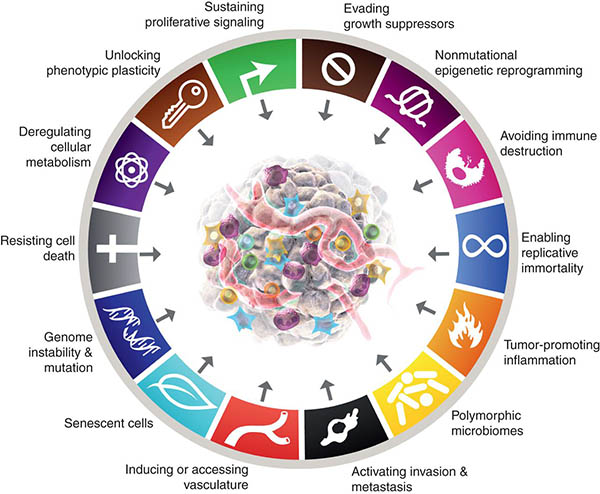
\includegraphics[width=0.85\textwidth]{resources/images/Hallmarks-of-Cancer.jpg}
    \caption{Hallmarks of Cancer}
    \label{fig:hallmarks_of_cancer}
\end{figure}
Another organization principle for cancerous diseases is found in the Hallmarks of cancer,~\ref{fig:hallmarks_of_cancer}, of Douglas Hanahan and Robert Weinberg~\cite{10.1158/2159-8290.CD-21-1059}. They describe a set of functional capabilities, eight hallmark capabilities, and two enabling characteristics commonly acquired by cancer cells. They contribute to their ability to grow uncontrollably, evade the immune system, and metastasize. These hallmarks are sustaining proliferative signaling, evading growth suppressors, avoiding immune destruction, enabling replicative immortality, tumor-promoting inflammation, activating invasion and Metastization, inducing or accessing vasculature, genome instability and mutation, resisting cell death, deregulating cellular metabolism. These Hallmarks of Cancer together contribute to the development and progression of cancer and provide targets for therapeutic intervention and research efforts aimed at understanding and treating the disease. 

In our model, we see many of the capabilities incorporated. Proliferative signaling only relies on the tumor cells themselves and not on typically other hormones or molecules, allowing them to proliferate rapidly without external growth signals. Immune destruction and induced cell death are avoided, optimizing them to survive and accumulate genetic mutations that promote tumor growth. The tumor cells can invade the surrounding tissue, modeled by the extracellular matrix.

\subsection{Mathematical Methods in Oncology}
Mathematical methods and models in Oncology play a crucial role in analyzing, understanding, and predicting cancer development. Since the objective of this research underlies complex and intricate biochemical systems and mechanisms, many models exist that find their respective applications in distinct areas of this research field. These methods can be coarsely divided into three sections: continuous, discrete, and hybrid models~\cite{BEKISZ2020101198}; for describing tumor growth, exponential and logistic growth models are often used, the latter allowing limiting factors to play a role during modeling. These methods are a subclass of the differential equations approach, which bases their functionality on an ordinary or partial differential equation, studying the continuous approach. Like our model, they are not limited to only one equation but can include many, incorporating systematic dependencies on other factors. These models generally deal with continuous quantities like densities or concentrations, for example, spatial and temporal nutritional supply or drug concentration, as well as their effects on the affected area over time. Discrete models use discrete entities to describe the behavior of tumor cells and their interactions with surrounding tissue. They allow us to model a wide range of biological and chemical processes which are hard to describe continuously. Commonly used types in mathematical oncology are, for example, Cellular Automata or Agent-Based Models. Cellular Automata represents cells as entities with states on a grid, with each cell being allowed to change states according to a set of rules based on its own current state and the states of the neighbors.

In contrast, Agent-Based Models enable the differentiation of cell types and allow movement that is not restricted to a grid, implementing complex mechanics at cell-cell or cell-environment levels. Using these discrete models allows researchers to focus on biological effects during modeling, which are hard to describe in continuous models. With these approaches, we can simulate genetic and evolutionary events. For example, they are studying the genetic alternations of tumor cells or the interaction between healthy and cancerous cells.

Hybrid models combine both methods above, using continuous and discrete approaches. Like in the model proposed by Franssen et al.~\cite{franssen_mathematical_2019} or Anderson et al.~\cite{anderson_continuous_1998}, these approaches allow to incorporate the exactness of continuous models with a wide range of biological effects described by discrete models.

However, not all models try to model tumor growth; others are concerned with optimality regarding drug dosages or radiation exposition, offering personalized treatment, or Machine Learining and Data Mining methods analyzing large datasets to identify patterns and predict outcomes. The latter method may be used in all kinds of applications, for example, spacial or temporal cancer development, as well as drug dosage optimization for individual patients. Putting all these methods together gives us a powerful toolbox to simulate and understand cancer biology. As the last years have shown, they are applied in a wide range of areas, offering insight into all areas of cancer research. Therefore, it is essential to come up with methods and evaluate their usefulness and meaningfulness in different research areas.